\section{Klassifizierung von Kommunikationssystemen S. 3}

\subsection{Klassifizierung nach Übertragungsdistanz S.4}
\begin{table}[H]
	\centering
	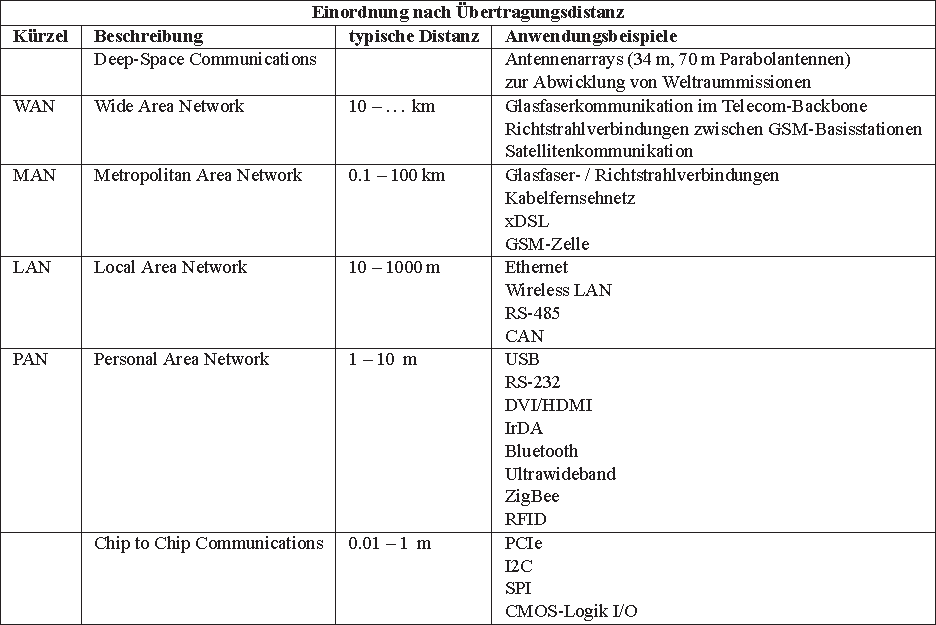
\includegraphics[width=.83\textwidth]{content/02_Klassifizierung/Tabelle1_3.pdf}
\end{table}
\subsection{Klassifizierung nach Zugriffsverfahren S.4}
\begin{table}[H]
	\centering
	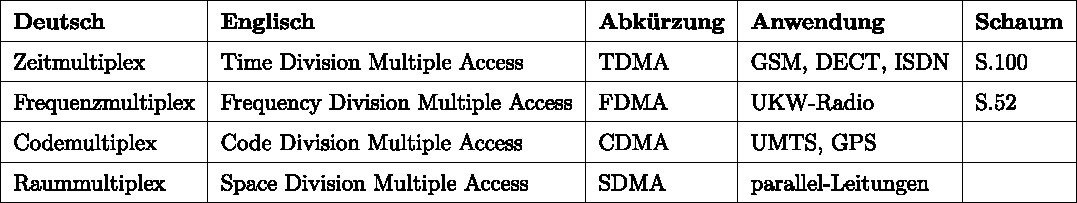
\includegraphics[width=.85\textwidth]{content/02_Klassifizierung/multiplexingverfahren.pdf}
\end{table}
\subsection{Klassifizierung nach Frequenzbereich S.6}
\begin{table}[H]
	\centering
	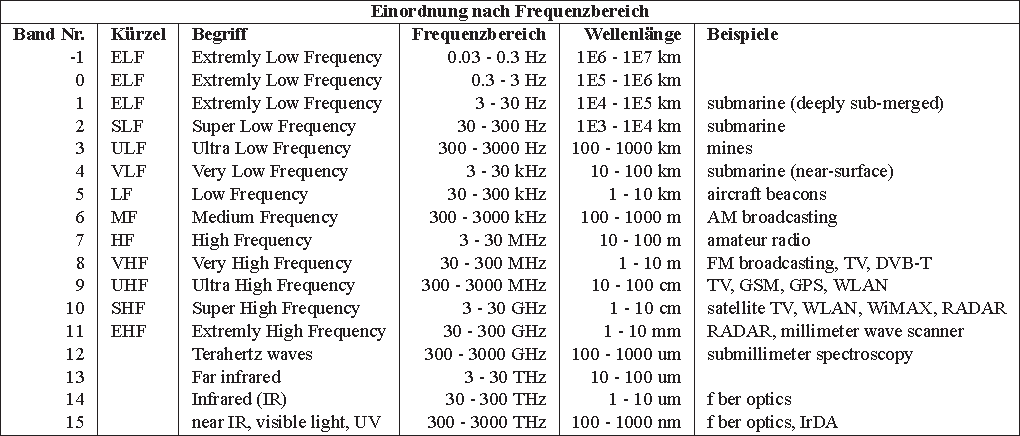
\includegraphics{content/02_Klassifizierung/Tabelle1_5.pdf}
\end{table}
\subsection{Klassifizierung nach Adressierung S.6}
\begin{table}[H]
	\centering
	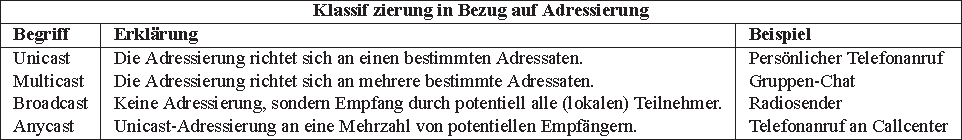
\includegraphics{content/02_Klassifizierung/Tabelle1_6.pdf}
\end{table}


\newpage
% \input{content/02_Signale/02_Signale}